\section{Literature Overview}

% --- Slide 1: The FIM Landscape ---
\begin{frame}[t]{The Evolution of FIM Environments}
    \vspace{0.2cm}
    Before addressing the HTT, we must categorize how FIM has adapted to shifting hardware constraints:
    
    \vspace{0.4cm}
    \renewcommand{\arraystretch}{1.3}
    \centering
    \begin{tabularx}{\textwidth}{l l l >{\raggedright\arraybackslash}X}
        \rowcolor{SecondaryColor!20}
        \textbf{Era} & \textbf{Algorithm} & \textbf{Storage} & \textbf{Main Bottleneck} \\ \hline
        Classic & Apriori & Local RAM & Memory Capacity \\
        Distributed & PFP (Hadoop) & HDFS (Disk) & \textbf{Network \& Disk I/O} \\
        \textbf{Modern} & \textbf{Spark} & \textbf{RDD (RAM)} & \textbf{CPU (Search)} \\ \hline
    \end{tabularx}

    \vspace{0.6cm}
    \begin{itemize}
        \item \textbf{The Shift:} Spark's RDD persistence effectively "solved" the I/O problem.
        \item \textbf{The New Reality:} When data is already in RAM, the time spent traversing pointer-heavy structures becomes the dominant cost.
    \end{itemize}
\end{frame}

% --- Slide 2: The Migration from MapReduce to Spark ---
\begin{frame}[t]{Architectural Migration: Hadoop to Spark}
    \begin{itemize}
        \item \textbf{Hadoop Era (PFP, PARMA, FPC/DPC):}
        \begin{itemize}
            \item \small MapReduce algorithms faced high latency due to launching new jobs for every iteration.
            \item \small \textbf{Costly I/O:} Constant disk read/write operations for intermediate results.
        \end{itemize}
        \item \textbf{The Spark Era (YAFIM, R-Apriori):}
        \begin{itemize}
            \item \small \textbf{YAFIM:} The pioneer Spark-based Apriori. It eliminated disk I/O, proving that in-memory RDD computation is 25x faster.
        \end{itemize}
    \end{itemize}

    \begin{center}
        \begin{tikzpicture}[scale=0.85]
            % X-Axis
            \draw[thick, ->] (0,0) -- (6,0) node[right, font=\tiny] {Time};
            % Hadoop Bar
            \draw[fill=red!20, draw=red] (0.5,0.2) rectangle (5.5,0.6) node[pos=.5, font=\tiny] {Hadoop Latency};
            % Spark Bar
            \draw[fill=green!20, draw=green!60!black] (0.5,-0.6) rectangle (1.2,-0.2) node[pos=.5, font=\tiny] {Spark};
            % Speedup Annotation
            \draw[<->, thick, SecondaryColor] (1.3,-0.4) -- (5.5,-0.4);
            \node[font=\scriptsize, SecondaryColor, below] at (3.4,-0.4) {$\approx 25\times$ Faster};
        \end{tikzpicture}
    \end{center}

    \begin{alertblock}{Transition Summary}
        \footnotesize Shift from \textbf{Disk Latency} to \textbf{In-Memory Search Speed}.
    \end{alertblock}
\end{frame}

% --- Slide 3: Pruning Strategy ---
\begin{frame}[t]{Pruning Strategies}
    \begin{itemize}
        \item \textbf{The Goal:} Reduce the number of candidate itemsets that need to be counted.
        \item \textbf{The Logic:}
        \begin{itemize}
            \item \small If an itemset is identified as non-frequent through pruning, it is discarded instantly.
            \item \small Only the remaining "potential" candidates proceed to the actual counting phase.
        \end{itemize}
    \end{itemize}

    \begin{center}
        \begin{tikzpicture}[scale=0.8]
            \draw[thick] (0,0) rectangle (4,0.3);
            \foreach \x in {0.5,1.2,2.8,3.5} \fill[AlertColor] (\x-0.1,0.05) rectangle (\x+0.1,0.25);
            \draw[->, thick, red] (1.2,-0.5) -- (1.2,-0.1) node[midway, left, font=\tiny] {Check};
            \node[font=\tiny, right] at (1.4,-0.4) {Result: Non-frequent? $\to$ Pruned};
        \end{tikzpicture}
    \end{center}
    
    \begin{alertblock}{Focus}
        \footnotesize Pruning effectively reduces the total \textbf{candidate count} before the search begins.
    \end{alertblock}
\end{frame}

% --- Slide 4: Data Structure Innovations (Balanced Height Version) ---
\begin{frame}[t]{Data Structures in Related Work}
    Beyond global pruning, researchers explored local memory-mapping:
    
    \begin{itemize}
        \item \small \textbf{Boolean Vectors (DFIMA):} Uses bitwise matrix pruning to handle candidates efficiently within Spark.
        \item \small \textbf{Array Vectors (Yang et al.):} Maps the database into contiguous memory for fast parallel iteration.
        \item \small \textbf{Ultrametric Trees (FiDoop):} Uses the \textit{FIU-Tree} to provide a more compressed representation.
    \end{itemize}

    \vspace{0.1cm}
    \begin{columns}[T]
        \begin{column}{0.48\textwidth}
            \begin{alertblock}{Pointer-Based (Legacy)}
                \scriptsize \centering
                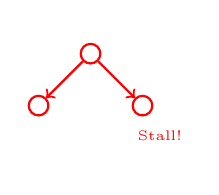
\begin{tikzpicture}[scale=1.1]
                    \tikzset{every node/.style={draw, circle, inner sep=2.5pt}}
                    \tikzset{every path/.style={->,red,thick}}
                    
                    \node (a) at (0,0.6) {};
                    \node (b) at (-0.6,0.0) {};
                    \node (c) at (0.6,0.0) {};
                    
                    \draw (a) -- (b); 
                    \draw (a) -- (c);
                    
                    \node[draw=none, circle=none, red, font=\tiny] at (0.8,-0.35) {Stall!};

                    \path (0,0.5) -- (0,0.9); 
                \end{tikzpicture}\\
                Memory Fragmentation
            \end{alertblock}
        \end{column}
        
        \begin{column}{0.48\textwidth}
            \begin{alertblock}{Direct Access (Proposed)}
                \scriptsize \centering
                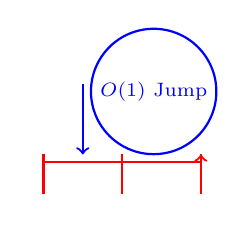
\begin{tikzpicture}[scale=1.0]
                    \draw (0,-0.4) grid (2,0.1);
                    \draw[->,blue,thick] (0.5,1.0) -- (0.5,0.1);
                    \node[blue, font=\scriptsize] at (1.4,0.9) {$O(1)$ Jump};
                    
                    \path[use as bounding box] (-0.2,-0.6) rectangle (2.2,1.2);
                \end{tikzpicture}\\
                Cache-Friendly
            \end{alertblock}
        \end{column}
    \end{columns}
\end{frame}

% --- Slide 5: The Remaining Challenge ---
\begin{frame}[t]{The Remaining Challenge}
    \begin{itemize}
        \item \textbf{The Progress:} Systems have moved from slow Disk I/O (Hadoop) to fast In-Memory RDDs (Spark).
        \item \textbf{The Success:} Modern techniques already use \textbf{Pruning} to reduce the number of candidates.
        \item \textbf{The Problem:} Even with fewer candidates, searching for itemsets inside an RDD partition is still the bottleneck.
    \end{itemize}

    \vspace{1.0cm}
    \begin{alertblock}{The Main Question}
        \centering
        \large \textit{"If the data is already in RAM, why is the search inside the partition still the bottleneck?"}
    \end{alertblock}
\end{frame}
